


\section{Code Availability and Data Management Plan}

The codebase for this thesis, including scripts for data preprocessing, model training, evaluation, and visualization, is available on GitHub. 
Detailed instructions on the project structure, usage, and dependencies can be found in the \texttt{README.md} file within the repository and each directories.

Please refer to the following link for the project's code and the structure of the project's data management plan:

\href{https://github.com/didemd/mlclassification_exotoxins}{\texttt{https://github.com/didemd/mlclassification\_exotoxins}}

\paragraph{Google Colab Notebooks for Embedding Generation}

The protein embeddings used in this research were generated using Google Colab notebooks due to the computational resources required for the ProtT5 and ProstT5 protein language models. 
Below are the links to the specific Colab notebooks used for generating these embeddings:

\begin{itemize}
	\item \textbf{ProstT5 Embedding Generation:}
	
	 \url{https://colab.research.google.com/drive/1X4XO3et7Bjoc8T8qvfYVbeCp2N1FbolD}{\texttt{https://colab.research.google.com/drive/1X4XO3et7Bjoc8T8qvfYVbeCp2N1FbolD}}
	\item \textbf{ProtT5 Embedding Generation:}
	
	 \href{https://colab.research.google.com/drive/1TUj-ayG3WO52n5N50S7KH9vtt6zRkdmj?usp=sharing\#scrollTo=ZQotVM94S7NR}{\texttt{https://colab.research.google.com/drive/1TUj-ayG3WO52n5N50S7KH9vtt6zRkdmj?usp=sharing\#scrollTo=ZQotVM94S7NR}}
\end{itemize}

These notebooks provide a reproducible workflow for generating the protein embeddings used in this thesis.


\section{Data Exploration and Processing}

This appendix section provides supplementary tables related to the data exploration and processing steps discussed in the main text. Table~\ref{fig:mean_value_type} and Table~\ref{fig:mean_value_target} present the mean hydrophobicity and sequence length values for each exotoxin type and target, respectively. 
Additionally, Table~\ref{tab:glm_hydrophobicity_appendix} and Table~\ref{tab:glm_sequence_length_appendix} display the detailed results of the \gls{GLM}.


\begin{table}[ht]
	\centering
	\caption{This table summarizes the mean hydrophobicity and sequence length for each exotoxin type, including Type I, Type II, Type III, Type IV, and Unknown.}
	\begin{tabular}{lcc}
		\toprule
		Type      & Hydrophobicity & Sequence Length \\
		\midrule
		Type I    & -0.399536      & 239.869565      \\
		Type II   & -0.192125      & 329.469027      \\
		Type III  & -0.358247      & 448.009302      \\
		Type IV   & -0.440321      & 706.000000      \\
		Unknown   & -0.300758      & 607.857143      \\
		\bottomrule
	\end{tabular}
		\label{fig:mean_value_type}
\end{table}

\begin{table}[ht]
	\centering
	\caption{This table presents the mean hydrophobicity and sequence length values for the two major exotoxin targets: non-vertebrate and vertebrate.}
	\begin{tabular}{lcc}
		\toprule
		Target          & Hydrophobicity & Sequence Length \\
		\midrule
		Non-vertebrate  & -0.316875      & 460.656958      \\
		Vertebrate      & -0.345380      & 438.744681      \\
		\bottomrule
	\end{tabular}
	\label{fig:mean_value_target}
\end{table}

\begin{table}[ht]
	\centering
	\caption{This table provides the GLM regression results for hydrophobicity, including exotoxin type and target.}
	\begin{tabular}{lccccc}
		\toprule
		Variable & Coefficient & Std Err & z & P$>$|z| & [0.025, 0.975] \\
		\midrule
		Intercept                   & -0.3998 & 0.073 & -5.446 & 0.000 & [-0.544, -0.256] \\
		C(type)[T.Type\_II]          & 0.2075 & 0.076 & 2.720  & 0.007 & [0.058, 0.357]  \\
		C(type)[T.Type\_III]         & 0.0414 & 0.070 & 0.589  & 0.556 & [-0.096, 0.179] \\
		C(type)[T.Type\_IV]          & -0.0408 & 0.098 & -0.415 & 0.678 & [-0.233, 0.152] \\
		C(type)[T.Unknown]          & 0.0991 & 0.083 & 1.189  & 0.234 & [-0.064, 0.262] \\
		C(target)[T.Vertebrate]     & 0.0003 & 0.026 & 0.011  & 0.991 & [-0.051, 0.051] \\
		\bottomrule
	\end{tabular}
	\label{tab:glm_hydrophobicity_appendix}
\end{table}

\begin{table}[ht]
	\centering
	\caption{This table displays the GLM regression results for sequence length, detailing the influence of exotoxin type and target on sequence length. The coefficients, standard errors, p-values, and confidence intervals for each predictor are shown.}
	\begin{tabular}{lccccc}
		\toprule
		Variable & Coefficient & Std Err & z & P$>$|z| & [0.025, 0.975] \\
		\midrule
		Intercept                   & 233.6480 & 91.005  & 2.567 & 0.010 & [55.282, 412.014] \\
		C(type)[T.Type\_II]          & 92.5175  & 94.587  & 0.978 & 0.328 & [-92.869, 277.904] \\
		C(type)[T.Type\_III]         & 209.9339 & 87.112  & 2.410 & 0.016 & [39.198, 380.670]  \\
		C(type)[T.Type\_IV]          & 466.1304 & 121.725 & 3.829 & 0.000 & [227.554, 704.707] \\
		C(type)[T.Unknown]          & 374.2091 & 103.257 & 3.624 & 0.000 & [171.829, 576.589] \\
		C(target)[T.Vertebrate]     & 6.2216   & 32.219  & 0.193 & 0.847 & [-56.926, 69.369] \\
		\bottomrule
	\end{tabular}
	\label{tab:glm_sequence_length_appendix}
\end{table}


\section{ExoType}

This appendix section provides supplementary figures and tables of the ExoType predictor. 
Figures~\ref{fig:learning_curve_type_import}, \ref{fig:MCC_type_import}, \ref{fig:precision_recall_type_import}, and \ref{fig:confusion_matrix_type_import} illustrate the learning curves, MCC scores, precision-recall curves, and confusion matrices, respectively, for models trained on protein sequence-based embeddings. 
Figures~\ref{fig:pr_curve_fold_type}, \ref{fig:confusion_matrix_fold_type}, and \ref{fig:confusion_matrix_fold_type_2} present the precision-recall curves and confusion matrices for models trained on protein fold-based embeddings. 
Finally, Table~\ref{tab:appendix_metrics_type} summarizes the per-class evaluation metrics for different machine learning models used for ExoType prediction.

\begin{figure}[H]
	\centering
	\includegraphics[width=0.9\textwidth]{images/learning_curve_type_import.png}
	\caption{\small This figure shows the learning curves for Random Forest, Logistic Regression, SVM, KNN. They are trained using protein sequence-based embeddings for exotoxin type prediction along with redundancy reduction split.}
	\label{fig:learning_curve_type_import}
\end{figure}

\begin{figure}[H]
	\centering
	\includegraphics[width=0.9\textwidth]{images/MCC_type_import.png}
	\caption{\small This figure shows the MCC plot for Random Forest, Logistic Regression, SVM, KNN with error bars. They are trained using protein sequence-based embeddings for exotoxin type prediction along with redundancy reduction split. MCC is used here as an evaluation metric to assess the overall quality of the models.}
	\label{fig:MCC_type_import}
\end{figure}

\begin{figure}[H]
	\centering
	\includegraphics[width=0.9\textwidth]{images/precision_recall_type_import.png}
	\caption{\small This figure shows the precision recall curve plot for Random Forest, Logistic Regression, SVM, KNN. They are trained using protein sequence-based embeddings for exotoxin type prediction along with redundancy reduction split.}
	\label{fig:precision_recall_type_import}
\end{figure}

\begin{figure}[H]
	\centering
	\includegraphics[width=1.1\textwidth]{images/confusion_matrix_type_import.png}
	\caption{\small This figure shows multiclass confusion matrix for Random Forest, Logistic Regression, SVM, KNN. They are trained using protein sequence-based embeddings for exotoxin type prediction along with redundancy reduction split.}
	\label{fig:confusion_matrix_type_import}
\end{figure}

\begin{figure}[H]
	\centering\includegraphics[width=0.99\textwidth]{images/precisionrecallcurvetypefolds.png}
	\caption{\small Precision-Recall curve for protein fold based embeddings. In each plot, the x-axis represents Recall, and the y-axis represents Precision. Each plot has the Average Precision (AP) value of Type I, Type II, Type III, Type IV, Unknown. AP measures the area under the precision-recall curve. The area under the corresponding curves are a metric for model performance. Multiclass PR curves treat each class as a separate “positive” and measure performance in one vs all.}
	\label{fig:pr_curve_fold_type}
\end{figure}

\begin{figure}[H]
	\centering\includegraphics[width=0.99\textwidth]{images/confusionmatrixtypefolds1.png}
	\caption{\small This confusion matrix displays multicass classification protein fold based embeddings. For each graph, there are sixteen cells that represent the exotoxin type category: Type I, Type II, Type III, Type IV, Unknown. Each cell represents percentage of categories that have a certain true label and were predicted to be a certain class. The diagonal cells shows the correct predictions whereas off-diagonal cells (Type I, II errors) are incorrect predictions. Additionally, the cell shading darkens as the percentage values increase.}
	\label{fig:confusion_matrix_fold_type}
\end{figure}

\begin{figure}[H]
	\centering\includegraphics[width=0.99\textwidth]{images/confusionmatrixtypefolds2.png}
	\caption{\small This confusion matrix displays multicass classification protein fold based embeddings. For each graph, there are sixteen cells that represent the exotoxin type category: Type I, Type II, Type III, Type IV, Unknown. Each cell represents percentage of categories that have a certain true label and were predicted to be a certain class. The diagonal cells shows the correct predictions whereas off-diagonal cells (Type I, II errors) are incorrect predictions. Additionally, the cell shading darkens as the percentage values increase.}
	\label{fig:confusion_matrix_fold_type_2}
\end{figure}

\begin{table}[H]
	\centering
	\caption{This table summarizes the per-class evaluation metrics (MCC, accuracy, precision, recall, and F1-score) for several machine learning models used to predict ExoType. The models include Random Forest, Logistic Regression, SVM, KNN, Hierarchical RF, and Hierarchical SVM.}
	\resizebox{\textwidth}{!}{  
		\begin{tabular}{llccccc}
			\toprule
			Model & Class & MCC & Accuracy & Precision & Recall & F1-Score \\
			\midrule
			\multirow{5}{*}{Random Forest} 
			& Type I   & 0.0000 & 0.9906 & 0.0000  & 0.0000  & 0.0000  \\
			& Type II  & 0.5446 & 0.9390 & 0.8750  & 0.3684  & 0.5185  \\
			& Type III & 0.5043 & 0.8779 & 0.8750  & 0.9943  & 0.9309  \\
			& Type IV  & 0.7037 & 0.9906 & 1.0000  & 0.5000  & 0.6667  \\
			& Unknown  & 0.3164 & 0.9484 & 0.6667  & 0.1667  & 0.2667  \\
			\midrule
			\multirow{5}{*}{Logistic Regression} 
			& Type I   & 0.4953 & 0.9906 & 0.5000  & 0.5000  & 0.5000  \\
			& Type II  & 0.4706 & 0.9249 & 0.6154  & 0.4211  & 0.5000  \\
			& Type III & 0.6625 & 0.8826 & 0.9689  & 0.8864  & 0.9258  \\
			& Type IV  & 0.5928 & 0.9671 & 0.3636  & 1.0000  & 0.5333  \\
			& Unknown  & 0.5309 & 0.9155 & 0.3846  & 0.8333  & 0.5263  \\
			\midrule
			\multirow{5}{*}{SVM} 
			& Type I   & 0.4015 & 0.9859 & 0.3333  & 0.5000  & 0.4000  \\
			& Type II  & 0.6864 & 0.9531 & 0.8000  & 0.6316  & 0.7059  \\
			& Type III & 0.7315 & 0.9108 & 0.9758  & 0.9148  & 0.9443  \\
			& Type IV  & 0.6586 & 0.9765 & 0.4444  & 1.0000  & 0.6154  \\
			& Unknown  & 0.6022 & 0.9390 & 0.4762  & 0.8333  & 0.6061  \\
			\midrule
			\multirow{5}{*}{KNN} 
			& Type I   & 0.7054 & 0.9953 & 1.0000  & 0.5000  & 0.6667  \\
			& Type II  & 0.6771 & 0.9531 & 0.8462  & 0.5789  & 0.6875  \\
			& Type III & 0.7192 & 0.9249 & 0.9301  & 0.9830  & 0.9558  \\
			& Type IV  & 0.6035 & 0.9812 & 0.5000  & 0.7500  & 0.6000  \\
			& Unknown  & 0.5260 & 0.9577 & 0.7143  & 0.4167  & 0.5263  \\
			\midrule
			\multirow{5}{*}{Hierarchical RF} 
			& Type I   & 0.0000 & 0.9906 & 0.0000  & 0.0000  & 0.0000  \\
			& Type II  & 0.6313 & 0.9484 & 0.9000  & 0.4737  & 0.6207  \\
			& Type III & 0.4792 & 0.8732 & 0.8706  & 0.9943  & 0.9284  \\
			& Type IV  & 0.0000 & 0.9812 & 0.0000  & 0.0000  & 0.0000  \\
			& Unknown  & 0.3985 & 0.9531 & 1.0000  & 0.1667  & 0.2857  \\
			\midrule
			\multirow{5}{*}{Hierarchical SVM} 
			& Type I   & 0.4953 & 0.9906 & 0.5000  & 0.5000  & 0.5000  \\
			& Type II  & 0.4950 & 0.9296 & 0.6667  & 0.4211  & 0.5161  \\
			& Type III & 0.7882 & 0.9343 & 0.9765  & 0.9432  & 0.9595  \\
			& Type IV  & 0.6586 & 0.9765 & 0.4444  & 1.0000  & 0.6154  \\
			& Unknown  & 0.6194 & 0.9437 & 0.5000  & 0.8333  & 0.6250  \\
			\bottomrule
		\end{tabular}
		}
		\label{tab:appendix_metrics_type}
\end{table}

\section{ExoTarget}
\label{sec:exotarget_appendix}

This appendix section provides figures and tables detailing the performance of the ExoTarget predictor. 
Figures~\ref{fig:sequence_learning_curves_import}, \ref{fig:mcc_plot_target_import}, \ref{fig:precision_recall_target_import}, and \ref{fig:confusion_matrix_target_import} illustrate the learning curves, MCC scores, precision-recall curves, and confusion matrices, respectively, for models trained on protein sequence-based embeddings for bacterial exotoxin targets. 
Figure~\ref{fig:pr_curve_fold} presents the precision-recall curves for models trained on protein fold-based embeddings. 
Finally, Table~\ref{tab:appendix_metrics_target} summarizes the per-class evaluation metrics for different machine learning models used for ExoTarget prediction.


\begin{figure}[H]
	\centering
	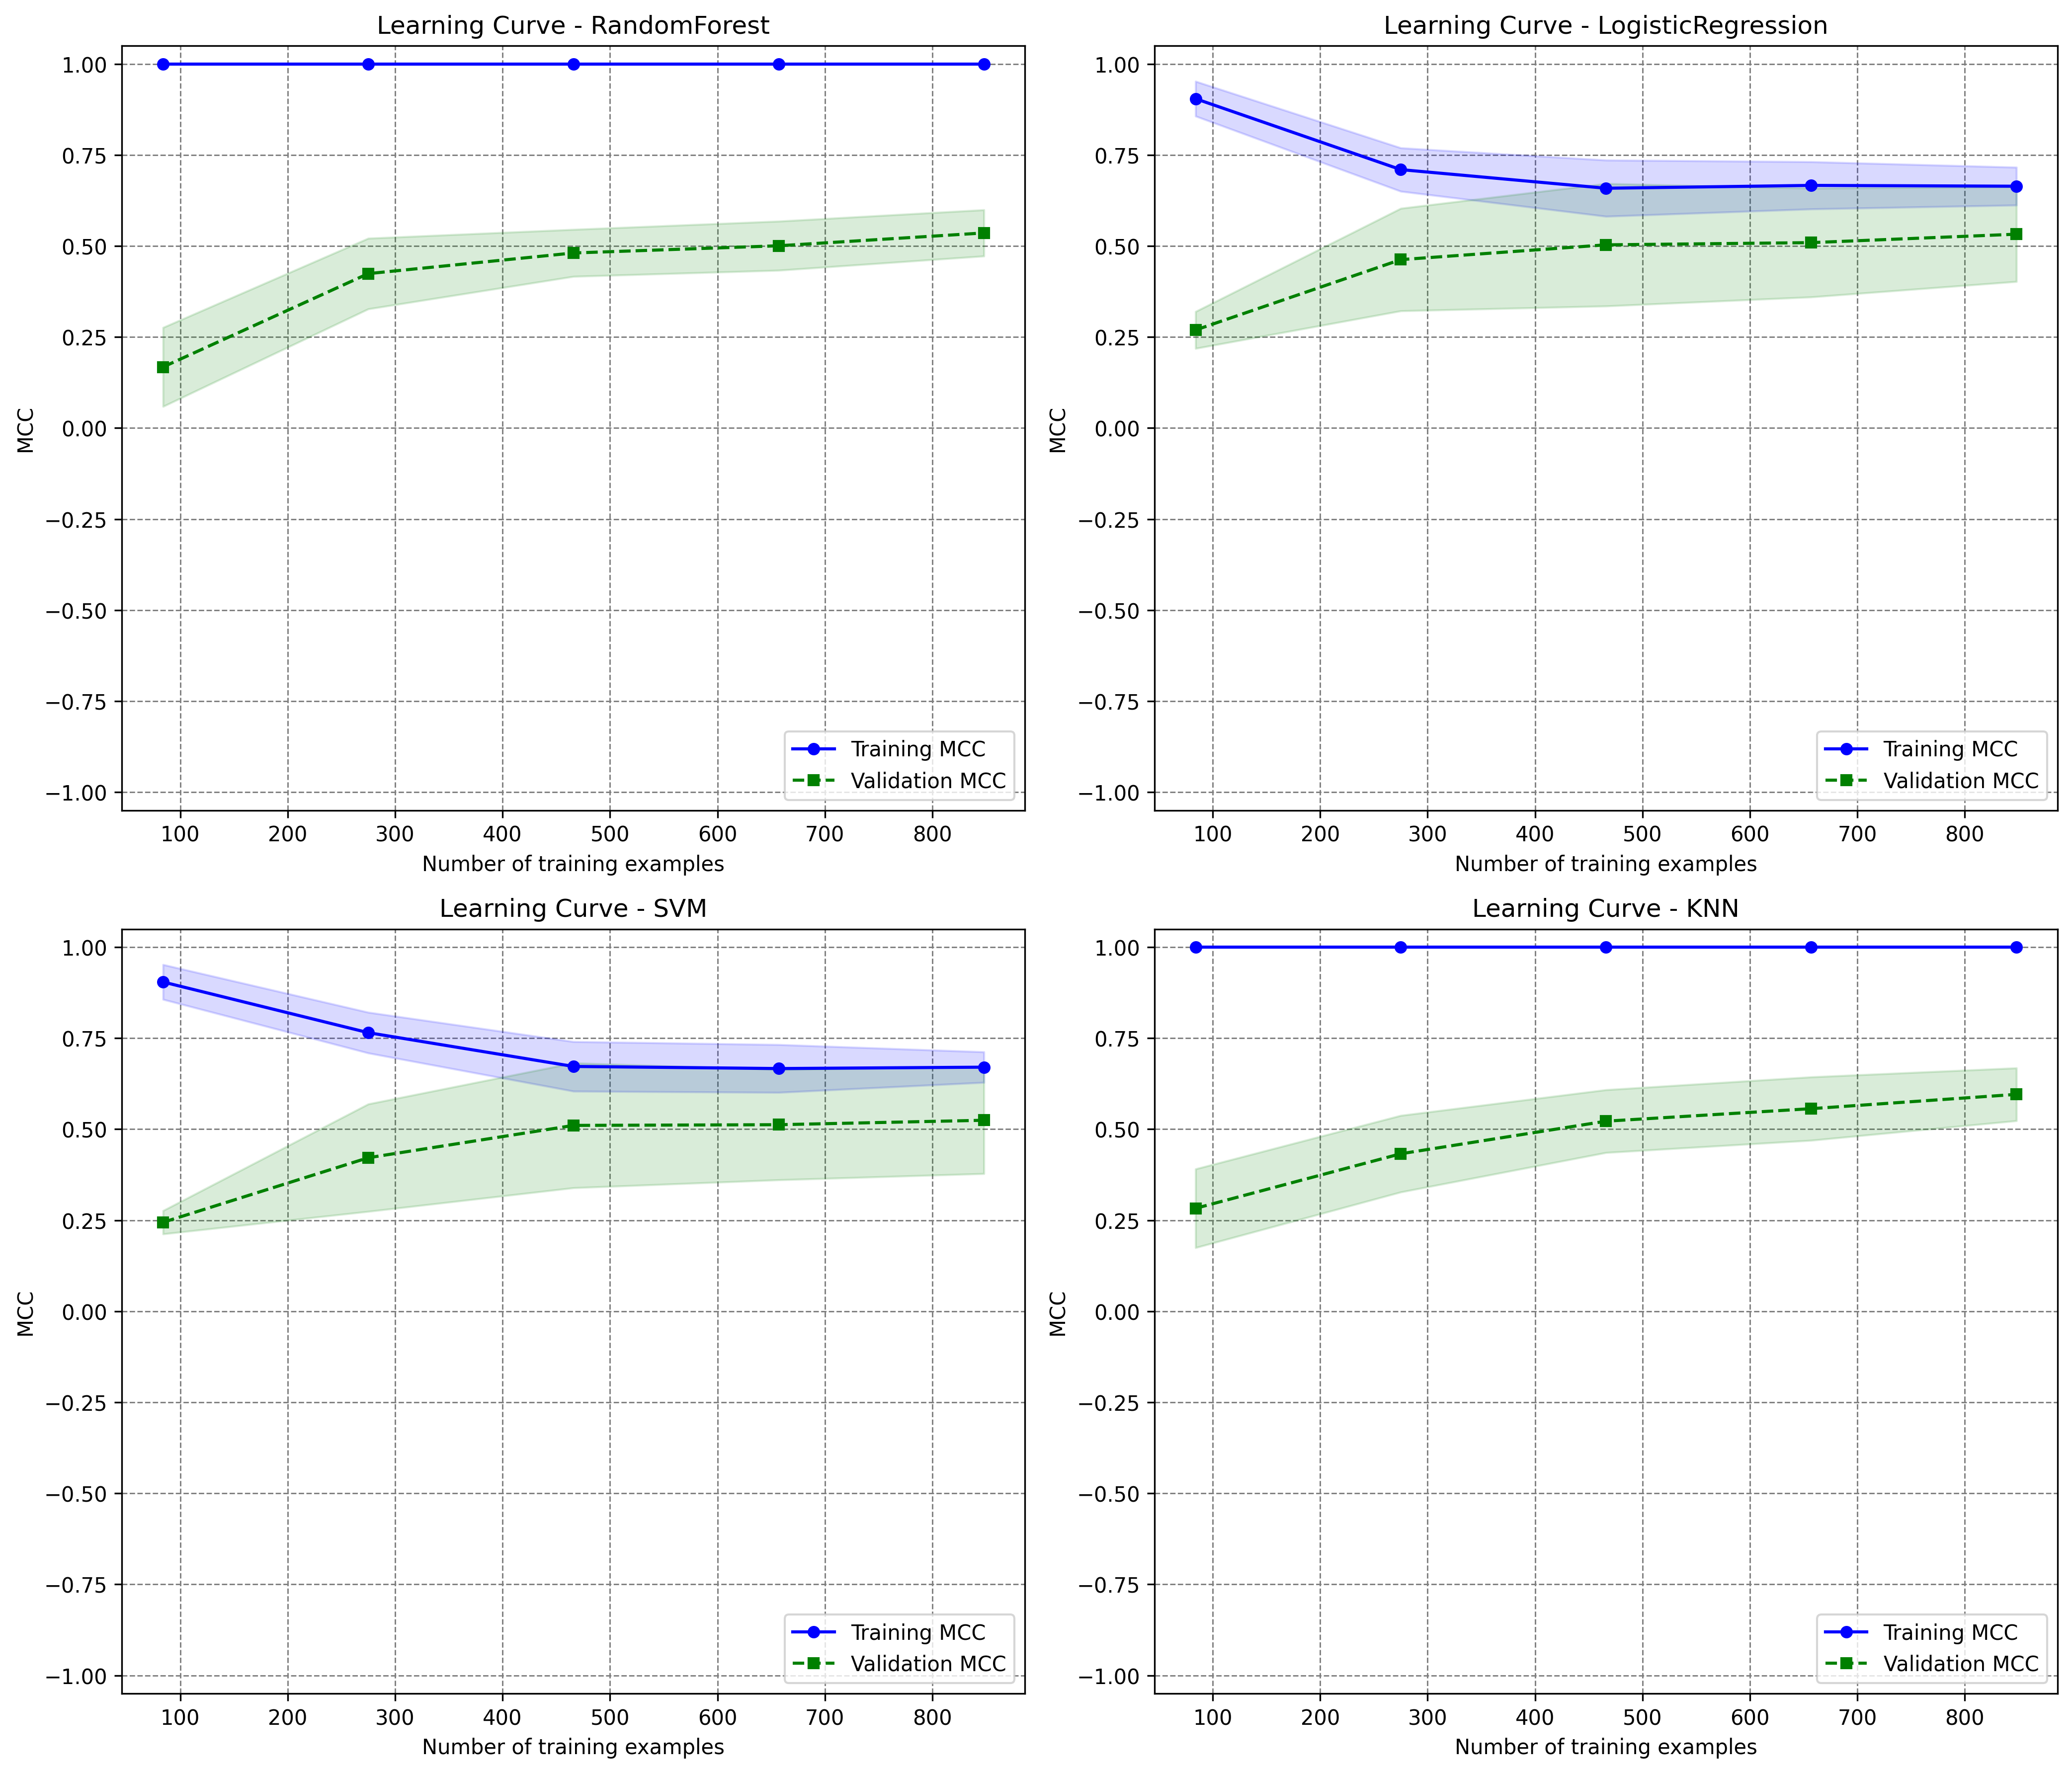
\includegraphics[width=0.9\textwidth]{images/2x2_learning_curves_import_test_target.png}
	\caption{\small This figure shows the learning curves for Random Forest, Logistic Regression, SVM, KNN. They are trained using protein sequence-based embeddings for exotoxin target prediction along with redundancy reduction split.}
	\label{fig:sequence_learning_curves_import}
\end{figure}

\begin{figure}[H]
	\centering\includegraphics[width=0.99\textwidth]{images/mcc_plot_target_import.png}
	\caption{\small This figure shows the MCC plot for Random Forest, Logistic Regression, SVM, KNN with error bars. They are trained using protein sequence-based embeddings for exotoxin target prediction along with redundancy reduction split. MCC is used here as an evaluation metric to assess the overall quality of the models.}
	\label{fig:mcc_plot_target_import}
\end{figure}

\begin{figure}[H]
	\centering\includegraphics[width=0.99\textwidth]{images/precision_recall_target_import.png}
	\caption{\small This figure shows the precision recall curve for Random Forest, Logistic Regression, SVM, KNN. They are trained using protein sequence-based embeddings for exotoxin target prediction along with redundancy reduction split.}
	\label{fig:precision_recall_target_import}
\end{figure}

\begin{figure}[H]
	\centering\includegraphics[width=0.99\textwidth]{images/confusion_matrix_target_import.png}
	\caption{\small This figure shows the confusion matrix for binary classification for Random Forest, Logistic Regression, SVM, KNN with error bars. They are trained using protein sequence-based embeddings for exotoxin target prediction along with redundancy reduction split.}
	\label{fig:confusion_matrix_target_import}
\end{figure}

\begin{figure}[H]
	\centering\includegraphics[width=0.99\textwidth]{images/precisionrecalltargetfolds.png}
	\caption{\small Precision-Recall Curve for Protein Fold-Based Embeddings for ExoTarget. In each plot, the x-axis represents Recall, and the y-axis represents Precision. The black dotted line shows a the chance baseline, which means the points above the diagonal line performs better than random guessing. The blue line depicts the Average Precision (AP). AP measures the area under the precision-recall curve. The area under the curve is a metric for model performance.}
	\label{fig:pr_curve_fold}
\end{figure}

\begin{table}[H]
	\centering
	\caption{This table summarizes the per-class evaluation metrics (MCC, accuracy, precision, recall, and F1-score) for several machine learning models used to predict ExoType. The models include Random Forest, Logistic Regression, SVM, KNN.}
	\begin{tabular}{llccccc}
		\toprule
		Model & Class & MCC & Accuracy & Precision & Recall & F1-Score \\
		\midrule
		\multirow{2}{*}{Random Forest} 
		& Non-Vertebrate & 0.5746 & 0.8404 & 0.8378 & 0.5254 & 0.6458 \\
		& Vertebrate & 0.5746 & 0.8404 & 0.8409 & 0.9610 & 0.8970 \\
		\midrule
		\multirow{2}{*}{Logistic Regression} 
		& Non-Vertebrate & 0.4966 & 0.7559 & 0.5393 & 0.8136 & 0.6486 \\
		& Vertebrate & 0.4966 & 0.7559 & 0.9113 & 0.7338 & 0.8129 \\
		\midrule
		\multirow{2}{*}{SVM} 
		& Non-Vertebrate & 0.517 & 0.7700 & 0.5581 & 0.8136 & 0.6621 \\
		& Vertebrate & 0.517 & 0.7700 & 0.9134 & 0.7532 & 0.8256 \\
		\midrule
		\multirow{2}{*}{KNN} 
		& Non-Vertebrate & 0.5634 & 0.8357 & 0.7857 & 0.5593 & 0.6535 \\
		& Vertebrate & 0.5634 & 0.8357 & 0.8480 & 0.9416 & 0.8923 \\
		\bottomrule
	\end{tabular}
	\label{tab:appendix_metrics_target}
\end{table}








































